\section{Tachometer på bil}

Formålet med tachometeret er at måle bilens nuværende hastighed, ved at måle omdrejningstallet på et af bilens forhjul. 
Tachometeret består af en TLE4905 \cite{lib:tle4905}
hallswitch, som fungerer ved at detektere magneter rettet i en bestemt retning. 
Kredsløbet er konstrueret således at hallswitchen trækker signalet til GND, når der detekteres en magnet. 
Kredsløbet bruger en meget lille strøm, målt til ca. 1.32mA, under tilstedeværelse af en magnet, uden er der målt en strøm på $520\mu A$. 
Med en forsyningsspænding på 5V bliver det til en effekt på 6.6mW, hvilket ikke betragtes som nogen EMC-mæssig trussel. 
Dog er der strømloops i systemet, som på tidspunkter vil være udsat for højfrekvente skift i strøm, hvilket er forsøgt forhindret ved at designe omtalte loops så små som muligt. 
Grundet det færdige prints størrelse, er det ikke muligt at placere det så tæt som muligt på hjulet som ønsket, hvorfor ledningerne ud til hall-switchen vil være snoede, således at common-mode støj undertrykkes.

\begin{figure}[h]
\centering
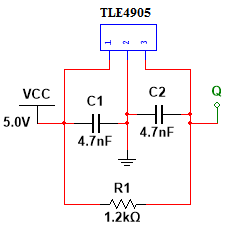
\includegraphics[scale=1]{../fig/billeder/tachometer_multisim.png}
\caption{Design af bilens tachometer i multisim.}
\label{fig:tachometer_multisim}
\end{figure}

Tachometeret er placeret i samme plastikhus, som bilens strømforsyning og motor, som begge er væsentlige støjkilder.
Det er af denne årsag at tachometeret er placeret ved bilens forhjul og ikke baghjul, hvor bilens motor sidder, da der derved opnås en højere afstand mellem støjkilde og støjfølsomt kredsløb.
Dog er tachometeret for så vidt ikke truet af støjoverkobling fra de øvrige kredsløb, da outputtet ligger fra 0V-5V, og der tælles på logisk LOW, ved Raspberry PI's GPIO. 
Dvs. at selvom der ligger 1V støj på outputtet, vil det ikke have nogen betydning for tachometerets præcision. 
Dette medfører at der skal rigtig meget støj til at påvirke outputtet af tachometeret. 

\clearpage